\chapter{食物的生产}\label{ch:g6:producing-our-food}

你的早餐桌上，没有一样东西是从野外找到的。面包
的小麦经过培育和种植；牛奶取自专门饲养的
牛群；酸奶则是由这些牛奶\emph{制成}的，制作者是
数以十亿计、肉眼看不见的微小\omterm{def:g6:exploring-our-environment:components}{生物}。人类
通过管理\omterm{def:g6:exploring-our-environment:components}{生物}来养活自己——培育它们、饲养它们，
并让其中最微小的一类为人所用。本章
带你参观这座食物工坊。

\section{种植与饲养}

\begin{definition}[农作物与畜牧]\label{def:g6:producing-our-food:farming}
人类的食物生产，在物质循环的
两个层级上管理\omterm{def:g6:exploring-our-environment:components}{生物}：
\begin{itemize}
  \item \emph{作物种植}\index{作物}：管理\omterm{def:g5:food-webs:roles}{生产者}
——小麦、马铃薯、蔬菜、水果——以获取它们的
        \omterm{def:g6:plants-are-producers:matter}{有机物}
        （见\cref{prop:g6:plants-are-producers:produce}）；
  \item \emph{畜牧养殖}\index{家畜}：管理
        \omterm{def:g5:food-webs:roles}{消费者}——牛、羊、猪、鸡——以获取它们的
        \omterm{def:g6:matter-from-food:production}{物质生产}
        （见\cref{def:g6:matter-from-food:production}）：牛奶、
        肉、蛋、羊毛。
\end{itemize}
农民管理的是本书反复遇到的\omterm{def:g6:exploring-our-environment:conditions}{条件}：\omterm{def:g6:decomposers-and-soil:soil}{土壤}
中的\omterm{prop:g4:what-plants-need:needs}{无机盐}供作物吸收（见\cref{rem:g4:what-plants-need:soil}），
为\omterm{def:g1:animals-around-us:animal}{动物}备料——这正是
\cref{pb:g6:matter-from-food:1}所记的整笔账，此处为有意而为。
\end{definition}

\begin{example}[麦田是什么]\label{ex:g6:producing-our-food:wheat}
麦田是一种经过管理的\omterm{def:g6:exploring-our-environment:components}{环境}
（见\cref{prop:g5:people-and-nature:managed}），专为一种
\omterm{def:g5:food-webs:roles}{生产者}而调整：\omterm{def:g6:decomposers-and-soil:soil}{土壤}经过补充养分和松土，以利于它的根，
播种时机与\cref{prop:g2:from-seed-to-plant:needs}中的
\omterm{def:g6:exploring-our-environment:conditions}{温度}需求相\omterm{def:g4:adapted-to-their-world:adaptation}{适应}；杂草作为争地的竞争者（见
\cref{ch:g6:how-plants-spread}）——须被排除在外。收获物是
\omterm{def:g1:plants-around-us:plant}{植物}的\omterm{def:g2:from-seed-to-plant:seed}{种子}储备：谷粒，是一百万株
永不再播种的小麦所备的“午餐”，被转运到面包房。
\end{example}

\begin{remark}[每一种食物都是生命周期中的一个阶段]\label{rem:g6:producing-our-food:stage}
从生物学角度看任何食物，它都是某种\omterm{def:g6:exploring-our-environment:components}{生物}的器官
或某个阶段：谷物与豆类是\omterm{def:g2:from-seed-to-plant:seed}{种子}储备；马铃薯是\omterm{ex:g4:plants-without-seeds:bulbtuber}{块茎}；
苹果则是为供人食用而生长的\omterm{prop:g3:flowers-fruits-seeds:transform}{果实}
（见\cref{exo:g6:how-plants-spread:12}）；牛奶是\omterm{prop:g3:sorting-living-things:groups}{哺乳动物}
的育幼之物（见\cref{def:g2:animals-grow-up:born}）；鸡蛋则是
一座装满养料的“育雏室”。食物生产，就是管理
\omterm{def:g2:born-grow-die:cycle}{生命周期}的艺术，使其所储备的养料能送上我们的餐桌。
\end{remark}

\section{看不见的劳动力：由微生物制成的食物}

\begin{definition}[发酵]\label{def:g6:producing-our-food:fermentation}
有些食物是通过让肉眼看不见的
——\emph{微生物}\index{微生物（食品）}——去加工一种原料而制成。它们的
取食使原料发生转化，这种转化
称为
\emph{发酵}\index{发酵}，人类已利用它
数千年，远在人们知道这些劳动者存在之前，
就已经如此。
\end{definition}

\begin{example}[面包为何膨胀]\label{ex:g6:producing-our-food:bread}
面包的生面团由面粉和水制成，再加上
\emph{酵母}\index{酵母}，一种单\omterm{def:g5:first-look-at-cells:cell}{细胞}\omterm{def:g6:decomposers-and-soil:decomposers}{真菌}
（见\cref{rem:g5:first-look-at-cells:onecelled}中已提到的此类
\omterm{def:g6:exploring-our-environment:components}{生物}）。\omterm{ex:g6:producing-our-food:bread}{酵母}以面粉中的糖为食，并释放
一种气体；气泡被困在有弹性的面团里，
使面团膨胀——面包师称之为“发起”。烤箱的热量
随后结束了这些劳动者的“轮班”；面包瓤上的
孔洞，就是\omterm{ex:g6:producing-our-food:bread}{酵母}留下的“签名”。
\end{example}

\begin{omfigure}
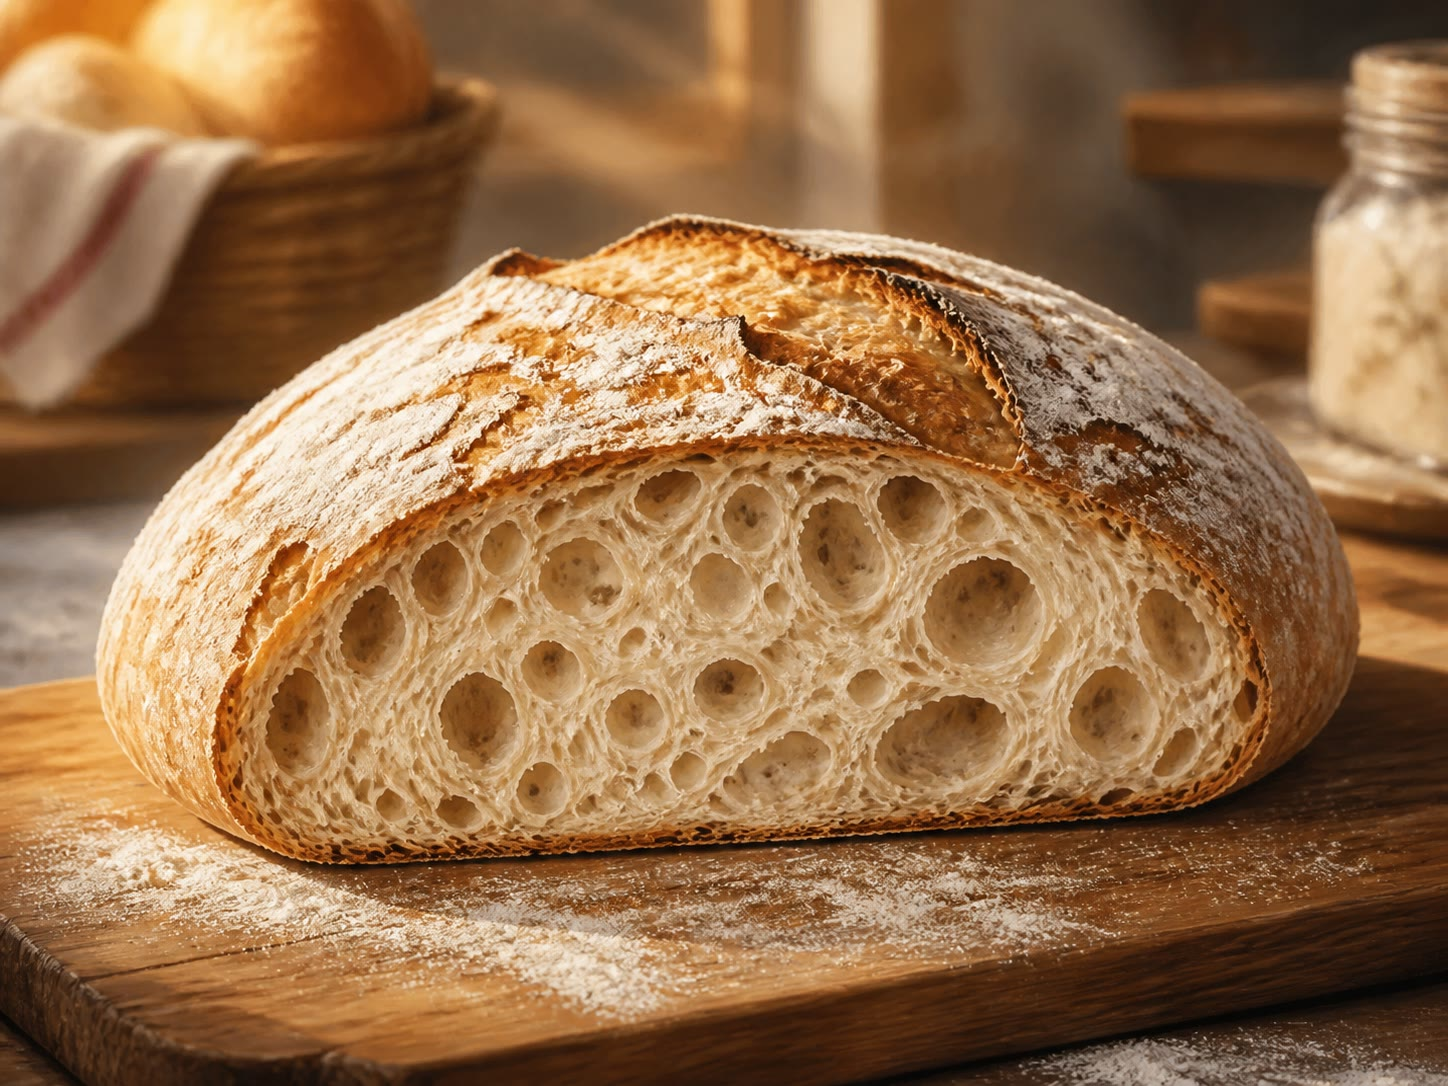
\includegraphics[width=0.58\linewidth]{images/book1/ai/g6-food-bread.jpg}

{\small 劳动者的“签名”，原样烘焙在面包中：面包瓤里的每一个
孔洞，都是\omterm{ex:g6:producing-our-food:bread}{酵母}吹出的气泡。}
\end{omfigure}

\begin{example}[牛奶变成酸奶和奶酪]\label{ex:g6:producing-our-food:yogurt}
接种了合适\omterm{def:g6:producing-our-food:fermentation}{微生物}的温牛奶，经过一夜便
凝结成酸奶：劳动者以牛奶中的糖为食，
并释放出一种酸，酸使牛奶凝固——清新的
酸味\emph{正是}这种酸。奶酪的开始与之相似，之后
则更进一步：凝乳经压制、加盐，熟成数月，
\omterm{def:g6:producing-our-food:fermentation}{微生物}在整个熟成期中仍在工作——奶酪的
孔洞、外皮和气味的浓烈程度，都是它们漫长“轮班”的记录。
\end{example}

\begin{remark}[有益与有害的微生物]\label{rem:g6:producing-our-food:goodbad}
\cref{def:g1:healthy-habits:germs}中的\omterm{def:g1:healthy-habits:germs}{病菌}，曾让人们警惕\omterm{def:g6:producing-our-food:fermentation}{微生物}；本章
则补充了另一半：
\emph{经过挑选的}\omterm{def:g6:producing-our-food:fermentation}{微生物}，在\emph{受控的}
\omterm{def:g6:exploring-our-environment:conditions}{条件}下工作，是我们最古老的“雇员”之一——面包、
酸奶、奶酪，还有醋缸，都离不开它们。这门手艺始终如一：
欢迎经过挑选的劳动者，并保持适合它们、而不利于
败坏者的\omterm{def:g6:exploring-our-environment:conditions}{条件}。加盐、冷藏、
干燥和烹饪，都是拒绝为不需要的\omterm{def:g6:producing-our-food:fermentation}{微生物}提供\omterm{def:g6:exploring-our-environment:conditions}{条件}的办法
（\cref{prop:g6:decomposers-and-soil:speed}在火腿上的作用，
与其在落叶堆上的作用完全相同）。
\end{remark}

\section{从田间到餐桌，说句实在话}

\begin{proposition}[餐桌上的代价]\label{prop:g6:producing-our-food:costs}
每一盘食物，都是经过管理的土地与\omterm{def:g6:exploring-our-environment:components}{生物}的产出，
并承载着它们的“账目”：
\begin{itemize}
  \item \omterm{def:g1:plants-around-us:plant}{植物}性食物距离光能只差一个层级；\omterm{def:g1:animals-around-us:animal}{动物}性
        食物先经由\omterm{def:g5:food-webs:roles}{消费者}，再承担
        \cref{prop:g6:matter-from-food:losses}所述的损耗
        （见\cref{exo:g6:matter-from-food:12}）；
  \item 可持续的生产，必须遵守
        \cref{prop:g5:people-and-nature:lasting}中的三条
        原则：养护\omterm{def:g6:decomposers-and-soil:soil}{土壤}、保护帮手、取用
        不超过更新的速度；
  \item 浪费则会使这一切付诸东流：被丢弃的食物
        所耗的土地、水和劳动，都白白浪费了。
\end{itemize}
\end{proposition}
\admitted

\begin{method}[读懂食物的来历]\label{met:g6:producing-our-food:read}
对厨房里的任何食物：
\begin{enumerate}
  \item 说出食物来自哪种\omterm{def:g6:exploring-our-environment:components}{生物}，以及取自它的哪个器官或哪个阶段
        （见\cref{rem:g6:producing-our-food:stage}）；
  \item 将它归入循环：\omterm{def:g5:food-webs:roles}{生产者}的物质、
        \omterm{def:g5:food-webs:roles}{消费者}的产物，还是\omterm{def:g6:producing-our-food:fermentation}{微生物}制成的？
  \item 若是\omterm{def:g6:producing-our-food:fermentation}{微生物}制成的，说出原料，以及这些“工人”
        改变了什么；
  \item 追溯至制造它的叶片
        （见\cref{met:g6:plants-are-producers:trace}）——这条线索
        最终仍总是指向光。
\end{enumerate}
\end{method}

\begin{example}[早餐中的方法]\label{ex:g6:producing-our-food:breakfast}
依此方法分析酸奶：（1）牛奶——奶牛哺育的
产物——经转化；（2）\omterm{def:g5:food-webs:roles}{消费者}的产物，
经\omterm{def:g6:producing-our-food:fermentation}{微生物}加工完成；（3）原料为牛奶，“工人”使其发酸并
凝结；（4）牛奶来自奶牛，奶牛吃草，草来自
光。三种\omterm{def:g6:exploring-our-environment:components}{生物}与数以十亿计的“工人”，
共处于一只小锅之中。
\end{example}

\section{练习}

\begin{exercise}[$\star$]\label{exo:g6:producing-our-food:1}
给出\omterm{def:g6:producing-our-food:farming}{作物种植}与\omterm{def:g6:producing-our-food:farming}{畜牧养殖}的定义，并指出各自管理的
是物质循环的哪一层。
\end{exercise}

\begin{exercise}[$\star$]\label{exo:g6:producing-our-food:2}
对每种食物，说出其\omterm{def:g6:exploring-our-environment:components}{生物}体及器官或阶段：
谷物、马铃薯、苹果、牛奶、卵。
\end{exercise}

\begin{exercise}[$\star$]\label{exo:g6:producing-our-food:3}
什么是\omterm{def:g6:producing-our-food:fermentation}{发酵}？说出两种\omterm{def:g6:producing-our-food:fermentation}{发酵}食品及其
原料。
\end{exercise}

\begin{exercise}[$\star$]\label{exo:g6:producing-our-food:4}
说明面包为何会膨胀：说出“工人”、其食物以及它
释放的物质，以及烤箱起了什么作用。
\end{exercise}

\begin{exercise}[$\star$]\label{exo:g6:producing-our-food:5}
什么使牛奶凝成酸奶？其酸味
来自何处？
\end{exercise}

\begin{exercise}[$\star$]\label{exo:g6:producing-our-food:6}
给出三种让不需要的\omterm{def:g6:producing-our-food:fermentation}{微生物}
无法获得所需\omterm{def:g6:exploring-our-environment:conditions}{条件}的方法，依据\cref{rem:g6:producing-our-food:goodbad}。
\end{exercise}

\begin{exercise}[$\star\star$]\label{exo:g6:producing-our-food:7}
一块麦田有意地满足
\cref{prop:g4:what-plants-need:needs}中的每项需求。请
将每项需求与农民的操作一一对应，
操作见\cref{ex:g6:producing-our-food:wheat}。
\end{exercise}

\begin{exercise}[$\star\star$]\label{exo:g6:producing-our-food:8}
请对奶酪逐步运用\cref{met:g6:producing-our-food:read}，
完整写出每一步。
\end{exercise}

\begin{exercise}[$\star\star$]\label{exo:g6:producing-our-food:9}
为什么冷藏能保存食物——而同样的
低温又会减慢堆肥的速度？同一原理，两处“厨房”，
请说出这一原理。
\end{exercise}

\begin{exercise}[$\star\star$]\label{exo:g6:producing-our-food:10}
请将\cref{def:g1:healthy-habits:germs}与本章相调和：
\omterm{def:g6:producing-our-food:fermentation}{微生物}怎样既是洗手要防的敌人，
又是酸奶的“工人”？
\end{exercise}

\begin{exercise}[$\star\star$]\label{exo:g6:producing-our-food:11}
运用\cref{prop:g6:producing-our-food:costs}，说明为何
一份被丢弃的火腿三明治，造成的浪费
比同重量被丢弃的面包更多。
\end{exercise}

\begin{exercise}[$\star\star\star$]\label{exo:g6:producing-our-food:12}
数千年来，面包师与酿酒师
在不知道\omterm{def:g6:producing-our-food:fermentation}{微生物}存在的情况下进行\omterm{def:g6:producing-our-food:fermentation}{发酵}。他们
实际管理的是什么，用
\cref{prop:g6:exploring-our-environment:decide}的术语
——他们的配方为何仍然有效？
\end{exercise}

\section{问题：班级面包坊}

\begin{problem}[{周末问题——一批面包，
从种子跟踪到面包片}]\label{pb:g6:producing-our-food:1}
为学校的集市，班级从零开始烘焙面包，
并从七月的麦田参观起，把\omterm{def:g6:exploring-our-environment:components}{生物}笔记一直记到
十一月的面包出炉为止。

\medskip\noindent\textbf{第一部分——麦田（七月）。}
\begin{enumerate}
  \item 农民展示成熟的小麦：“收获是
        \omterm{def:g1:plants-around-us:plant}{植物}打包好的午餐。”请解读这句话，
        结合\cref{def:g2:from-seed-to-plant:seed}——每粒谷物
        是什么，它又是为谁而打包的？
  \item 在哪些叶片中，借助什么原料，
        制造出了谷物的\omterm{def:g6:plants-are-producers:matter}{有机物}？
  \item 农民来年秋天只播种一部分收获，
        其余出售。请用\omterm{def:g2:born-grow-die:cycle}{生命周期}的术语，
        说出一粒小麦的两种去向。
  \item 收获后，麦田的\omterm{def:g6:decomposers-and-soil:soil}{土壤}会施用粪肥。这属于
        哪一条归还原则？它满足\omterm{def:g1:plants-around-us:plant}{植物}五项需求中的
        哪一项？
\end{enumerate}

\medskip\noindent\textbf{第二部分——面包房（十一月）。}
\begin{enumerate}[resume]
  \item 全班把面粉、水、盐和\omterm{ex:g6:producing-our-food:bread}{酵母}混合，
        然后把面团放在温暖的角落里。为什么要温暖？
        请像对待任何一位有生命的“工人”那样，回答\omterm{ex:g6:producing-our-food:bread}{酵母}的情况
        （\cref{prop:g6:decomposers-and-soil:speed} 中有此规律
        ）。
  \item 一小时后，面团已经膨胀到原来的两倍。试解释膨胀的原因：
        \omterm{ex:g6:producing-our-food:bread}{酵母}以什么为食，释放了什么，
        又是什么把这些气体困住了？
  \item 一组的面团被遗忘在一扇有穿堂风的冷窗旁，几乎不膨胀。
        请诊断原因，并说明两组
        无意中进行了哪一种
        公平测试的对比。
  \item 放入烤箱后，面包不再膨胀，而是定型。
        加热对这支“工人队伍”造成了什么影响，
        其在面包瓤中留下的标记又是什么？
\end{enumerate}

\medskip\noindent\textbf{第三部分——核算。}
\begin{enumerate}[resume]
  \item 沿环节逐一追溯这片成品面包，
        一直追溯到光。
  \item 集市还出售黄油三明治和火腿三明治。
        请将面包片、黄油和火腿，按其物质所经过的
        层级数从多到少排序，
        并指出哪一项损失最多，
        依据\cref{prop:g6:matter-from-food:losses}。
  \item 卖不掉的面团不丢弃，而是堆肥。
        请沿循环再往前追一步，追踪其\omterm{def:g6:plants-are-producers:matter}{有机物}，
        ——由谁获取，又流向何处？
  \item 用一句话作为笔记的结尾，句中须含有：
        \omterm{def:g5:food-webs:roles}{生产者}、\omterm{def:g5:food-webs:roles}{消费者}（如有）、\omterm{def:g6:producing-our-food:fermentation}{微生物}“工人队伍”，
        以及光。
\end{enumerate}
\end{problem}
